\section{Abelian Anyons III, Quantum Double Model I}

\subsection{Mutual Statistics of Toric Code Anyons}
We want to compute the mutual statistics of charge and flux statistics $e^{i\theta_{\text{em}}}$ in the Toric code. The strategy was to compare two paths, $\Gamma$ and $\Gamma'$ (see figure from last lecture) such that the paths look the same, but $\Gamma$ has a flux in the center of the path and $\Gamma'$ has a flux outside of it. By looking at the difference of the two processes, since the two paths ``look the same'', the uninteresting short-range contributions to the phase will cancel, leaving us with just $\theta_{\text{em}}$:
\begin{equation}
    \theta(\Gamma) - \theta(\Gamma') = \theta_{\text{em}}
\end{equation}
where $\theta(\Gamma), \theta(\Gamma')$ are the total phases accumulated by some sequence of local movement operators. Let's compute these and now see what we get. The simplest operator we can write down to move charges is $Z_j$ - the pauli-$Z$ operator on link $j$. This moves a charge from site $s$ to site $s'$ (and vise versa), as depicted in the figure from last lecture (the figure is slightly poorly notated; it should really depict movement of charges, as opposed to swapping the site labels. The precise action is captured in the anticommutation, or in the relations of Eq. \eqref{eq:applyZ}). We can see this from the anticommutation of $Z_j$ with $A_s, A_{s'}$.

Denote the initial state by $\ket{p_0, s}$. Let $\Gamma$ denote the process composed out of a sequence of $Z$ operators, which moves the charge $s$ along the path $\gamma$.

\begin{center}
    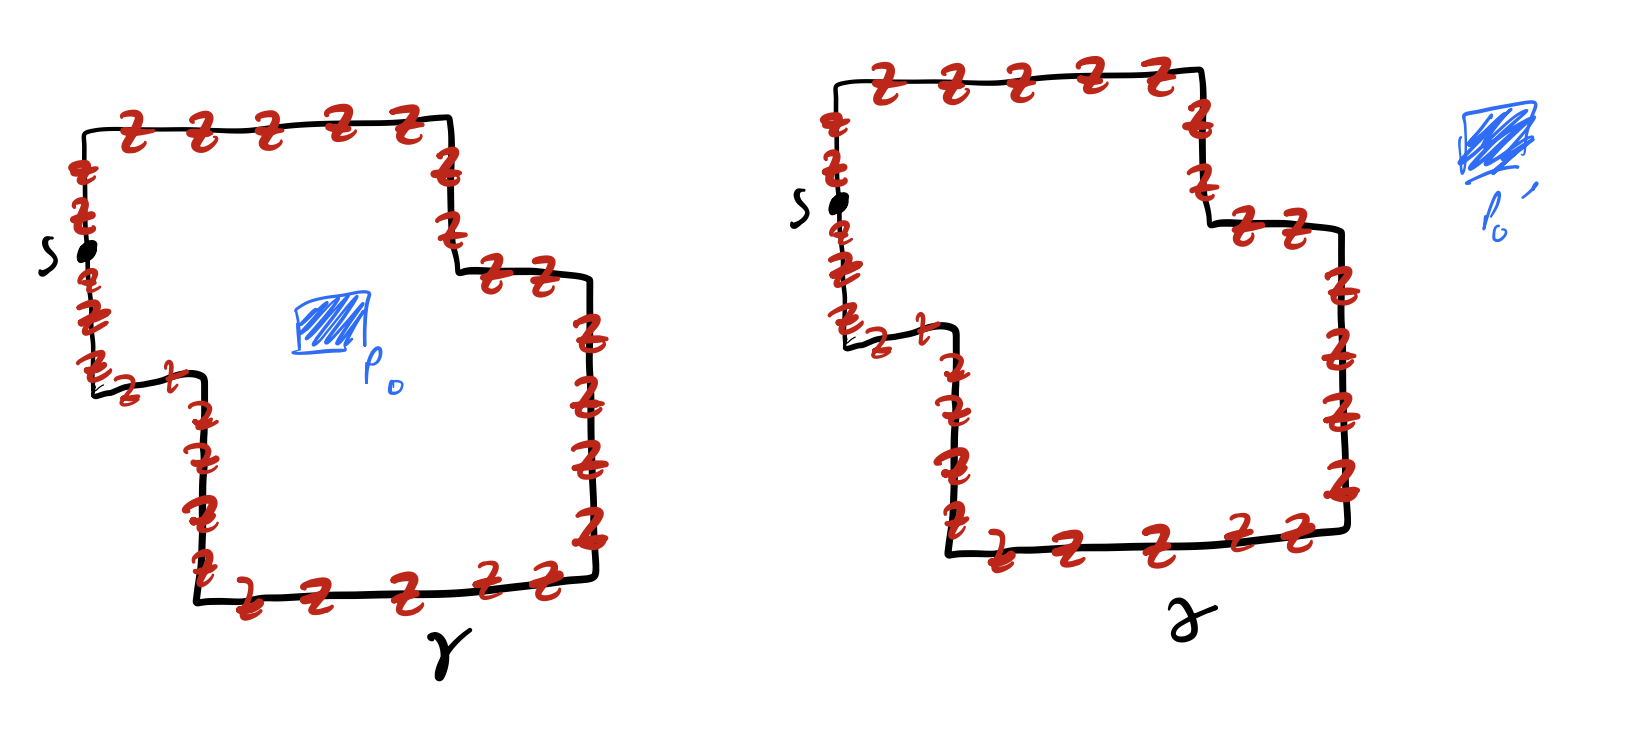
\includegraphics[scale=0.35]{Lectures/Images/lec6-twopaths.png}
\end{center}

By definition:
\begin{equation}
    \prod_{j \in \gamma}Z_j \ket{p_0, s} = e^{i\theta(\Gamma)}\ket{p_0, s}
\end{equation}
To figure out what $e^{i\theta(\Gamma)}$, we observe the operator identity:
\begin{equation}
    \prod_{j \in \gamma}Z_j = \prod_{p \in \text{int}(\gamma)}B_p
\end{equation}
Note that this is a kind of Stokes' theorem. We can use this identity to evalute $e^{i\theta(\Gamma)}$ - we're in business because there is exactly one $b_p = -1$ inside of $\gamma$:
\begin{equation}
    e^{i\theta(\Gamma)}\ket{p_0, s} = \prod_{p \in \text{int}(\gamma)}B_p\ket{p_0, s} = -\ket{p_0, s}
\end{equation}
Thus:
\begin{equation}
    e^{i\theta(\Gamma)} = -1
\end{equation}
We aren't quite done yet. We should compare this to the case where the flux is not in the center. Now, consider $\Gamma'$ which is an identical process save for the flux is on a plaquette $p_0'$ outside of the path $\gamma$. Then:
\begin{equation}
    e^{i\theta(\Gamma')}\ket{p_0', s} = \prod_{j \in \gamma}Z_j \ket{p_0', s} = \prod_{p \in \text{int}(\gamma)}B_p\ket{p_0', s} = +\ket{p_0', s}
\end{equation}
where the last equality follows since all $b_p = +1$ in the interior of the path (the only flux is outside). Thus:
\begin{equation}
    e^{i\theta(\Gamma')} = 1
\end{equation}
Therefore looking at the difference:
\begin{equation}
    e^{i\theta_m} = e^{i\theta(\Gamma)}e^{-i\theta(\Gamma')} = -1 \cdot 1 = -1
\end{equation}
Thus:
\begin{equation}
    \boxed{e^{i\theta_m} = -1}
\end{equation}
We compared two phases, one which was nontrivial and one which was trivial, and then the ratio gives us the interesting exchange statistic. 

Why was it important that we took the difference between these two paths/compared the two processes? We chose $Z$ as our movement operator, but someone else could have very well chosen $e^{i\phi}Z$ for any phase; then that random phase would contribute to $e^{i\theta(\Gamma)}$ and $e^{i\theta(\Gamma')}$. But crucially, it contributes in the exact same way to both of these, and hence does not contribute to the difference.

A couple remarks:
\begin{enumerate}
    \item The result does not depend on the microscopic details of the path $\gamma$. We expected this from what we know about the Berry phase, but also saw this clearly arise from the calculation itself. Moreover, $\theta_{\text{em}}$ does not depend on the choice of movement operator; we won't prove this in full generality, but we did remark how movement operators differing by a phase give the same result. In fact even if the movement operators look more starkly different, we find the same result.
    \item Mutual statistics are symmetric, and indeed we could swap the roles of the charges/fluxes and $Z/X$ and we would get the same results.
    \item According to the definition from last class, $e, m$ are indeed non-trivial anyons since $e^{i\theta_{\text{em}}} = -1$ (non-trivial mutual statistics, with each other).
    \item We could also ask what the mutual statistics of taking an $e$ particle around itself (or $m$ around itself). Then, its trivial to show that:
    \begin{equation}
        e^{i\theta_{\text{ee}}} = e^{i\theta_{\text{mm}}} = 1
    \end{equation}
    \item Note that an even number of charges/fluxes look like having no charges/fluxes at all. Actually, we have four types of ``sectors'' of excitations $\set{1, e, m, \e}$ with $1$ being even charges/fluxes, $e$ being odd charges even fluxes, $m$ being even charges odd fluxes, and $\e$ being odd charges and fluxes (you will study this one on the homework).
\end{enumerate}

\subsection{Connection between Abelian Anyons and String Operators}
We sketch the connection between mutual statistics and the algebra of string operators. In the previous section we gave a physically transparent way of computing mutual statistics, now we give the shortcut. Let $a, b$ be Abelian anyons, and let $W_a, W_b$ be associated string operators. $W_a$ creates an excitation $a$ at one end and its antiparticle $\bar{a}$ at its other end (in the toric code, the particles and antiparticles coincide). Consider paths $\gamma, \beta$, and then compare:
\begin{equation}
    W_a(\gamma)W_b(\beta)\ket{\Omega}, \quad  W_b(\beta)W_a(\gamma)\ket{\Omega}
\end{equation}

\begin{center}
    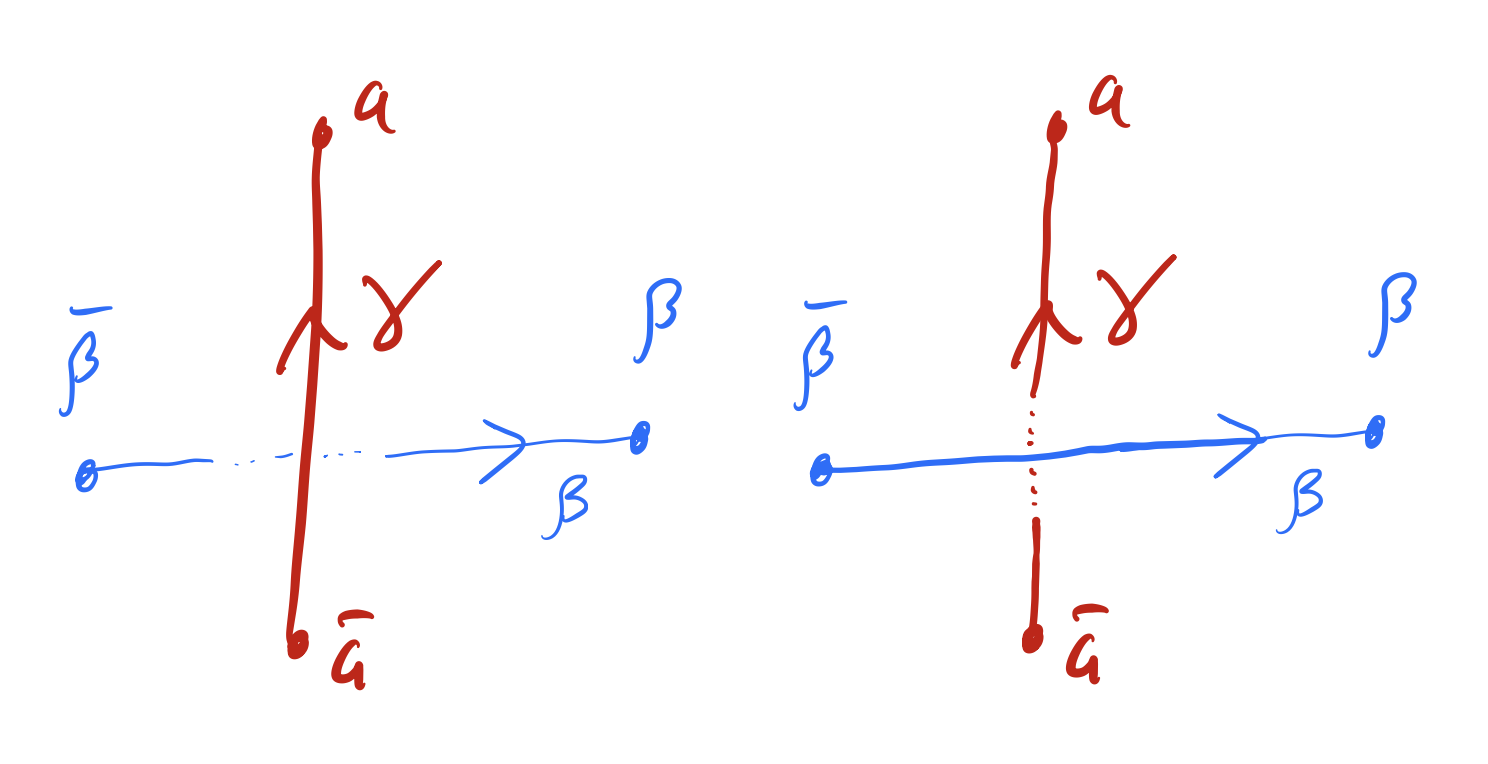
\includegraphics[scale=0.35]{Lectures/Images/lec6-stringoporder.png}
\end{center}

The claim is then:
\begin{equation}\label{eq:stringopmutualstat}
    W_a(\gamma)W_b(\beta)\ket{\Omega} = e^{i\theta_{ab}} W_b(\beta)W_a(\gamma)\ket{\Omega}
\end{equation}

For example, lets use $a = e, b = m$ on the toric code. The $b$-string is a string of $X$s that creates two fluxes on the end, and the $a$-string in a string of $Z$s that creates two charges on the end:

\begin{center}
    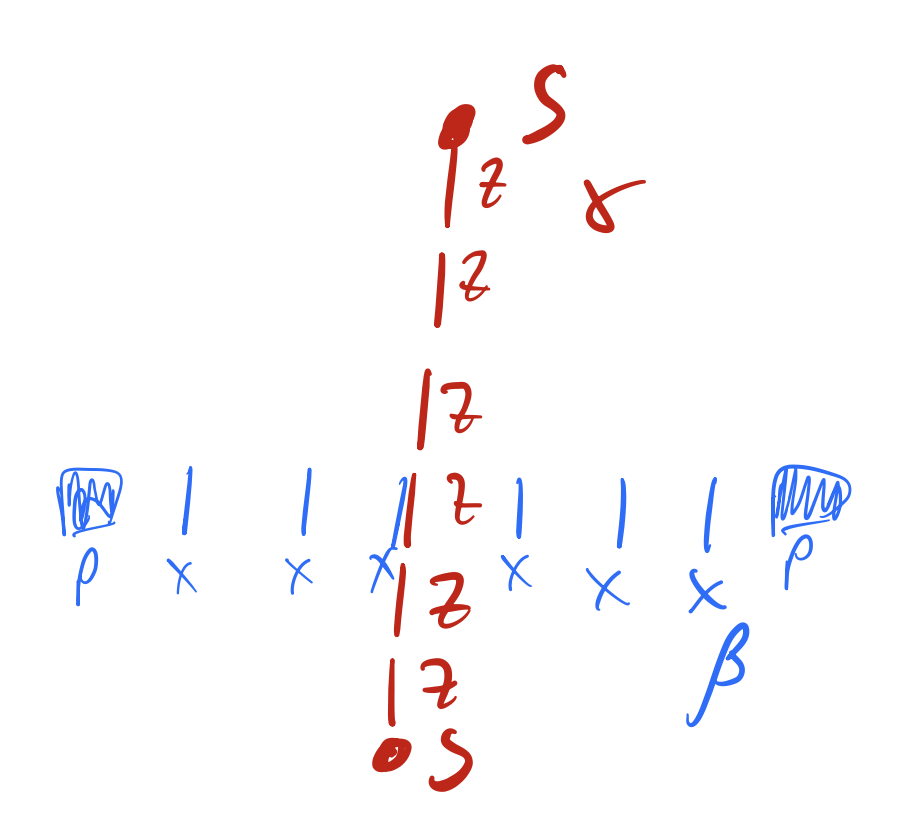
\includegraphics[scale=0.35]{Lectures/Images/lec6-stringopanticommute.png}
\end{center}

These two operators anticommute on the operator level:
\begin{equation}
    W_e(\gamma)W_m(\beta) = -W_m(\beta)W_e(\gamma)
\end{equation}
and hence also anticommute when acted upon the ground state. Thus:
\begin{equation}
    e^{i\theta_{\text{em}}} = -1
\end{equation}

Let us derive the general relation of Eq. \eqref{eq:stringopmutualstat}. On general grounds, we know that:
\begin{equation}
    W_a(\gamma)W_b(\beta)\ket{\Omega} = e^{i\theta}W_b(\beta)W_a(\gamma)\ket{\Omega}
\end{equation}
for \emph{some} phase $\theta$. This is because both of the states correspond to the creation of anyons on both sides - hence both states have the same 4 anyons ($a, \bar{a}, b, \bar{b}$) at the same locations. Hence they must describe the same physical state. To compute the phase, we multiply both the right and left hand side with a further string operator, $W_a(\gamma')$:
\begin{equation}
    W_a(\gamma')W_a(\gamma)W_b(\beta)\ket{\Omega} = e^{i\theta} W_a(\gamma')W_b(\beta)W_a(\gamma)\ket{\Omega}
\end{equation}

Graphically, the LHS/RHS look like:

\begin{center}
    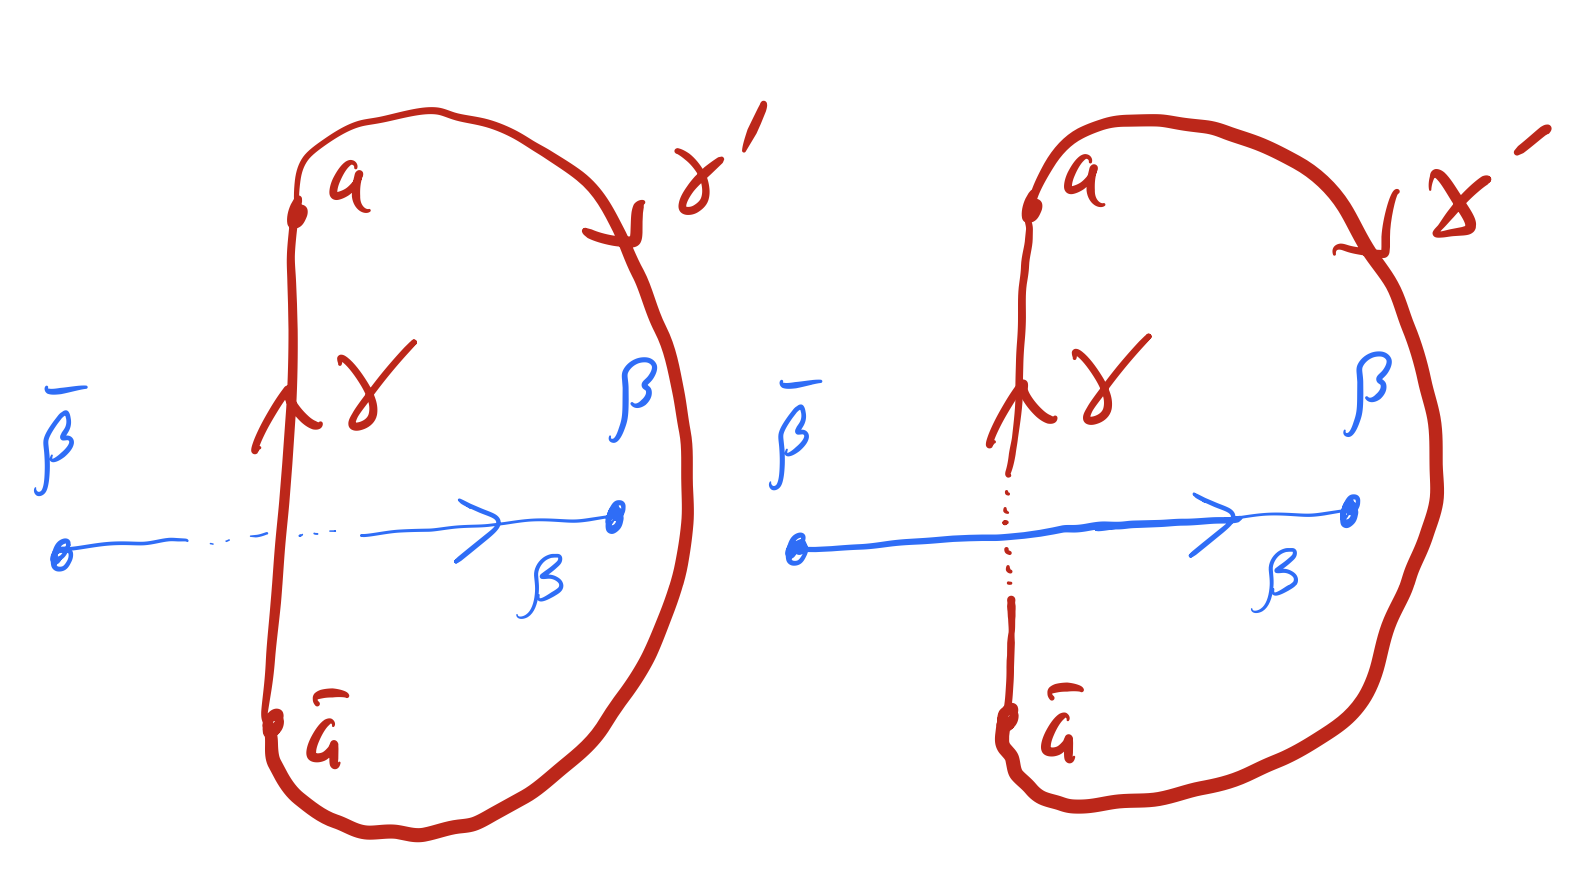
\includegraphics[scale=0.35]{Lectures/Images/lec6-braid.png}
\end{center}

The first thing we see at an algebraic level is that $W_a(\gamma')$ commutes with $W_b(\beta)$, as they act on non-overlapping places:
\begin{equation}
    W_a(\gamma')W_a(\gamma)W_b(\beta)\ket{\Omega} = e^{i\theta} W_b(\beta)W_a(\gamma')W_a(\gamma)\ket{\Omega}
\end{equation}
Now let's think about the two processes we have here. On the LHS, we have that $a$ braids around $b$ (we first create $b$ and then do the big loop). On the RHS, we first create $a, \bar{a}$ and do the big loop, and then create $b$ - $a$ follows the exact same path, but does $\emph{not}$ braid around $b$. Thus, we would conclude that the phase difference $\theta$ must be the topological Berry phase $\theta_{ab}$, as everything else cancels.

To summarize:
\begin{enumerate}[(a)]
    \item Abelian anyon excitations $\iff$ non-commuting flexible string operators (with the algebra of the SOs encoding the mutual statistics. On the HW, you will also see that the algebra of the SOs imply exchange statistics, but this will require looking at three string operators)
    \item Non commuting flexible string operators $\implies$ Robust GSD (on torus)
    \item Robust GSD $\implies$ robust quantum memory (can encode the qubit in the GSD).
\end{enumerate}
Thus any system with Abelian anyons has all these properties... it is harder to formulate the reverse statement, but easy counterexamples don't come to mind.

\subsection{Introduction to the Quantum Double Model}
The above concludes our discussion of abelian anyons and the toric code. We thus move onto the discussion of non-abelian anyons and the quantum double model. The reference is \texttt{quant-ph/9707021}. 

We can think of the quantum double model as the generalization of the toric code. It's not actually a single model, but a class of models, of which we specify a specific model by choice of a finite group $G$. The toric code corresponds to choosing $G = \ZZ_2$ (the simplest nontrivial choice). Looking a bit ahead, when we choose $G$ to be Abelian, the model will host Abelian anyons, but when we choose $G$ to be a non-Abelian group, the quantum double model will host non-Abelian anyon excitations.

What are non-Abelian anyons? In short, Abelian if we trap $n$ particles at $n$ sites have a unique physical state, vs. for non-Abelian anyons the same process results in a ground state with degeneracy. We will see that the braiding processes for these anyons will not be Abelian.

We have a local Hilbert space on each edge site of a lattice, with each edge Hilbert space having dimension $\abs{G}$. 

\begin{center}
    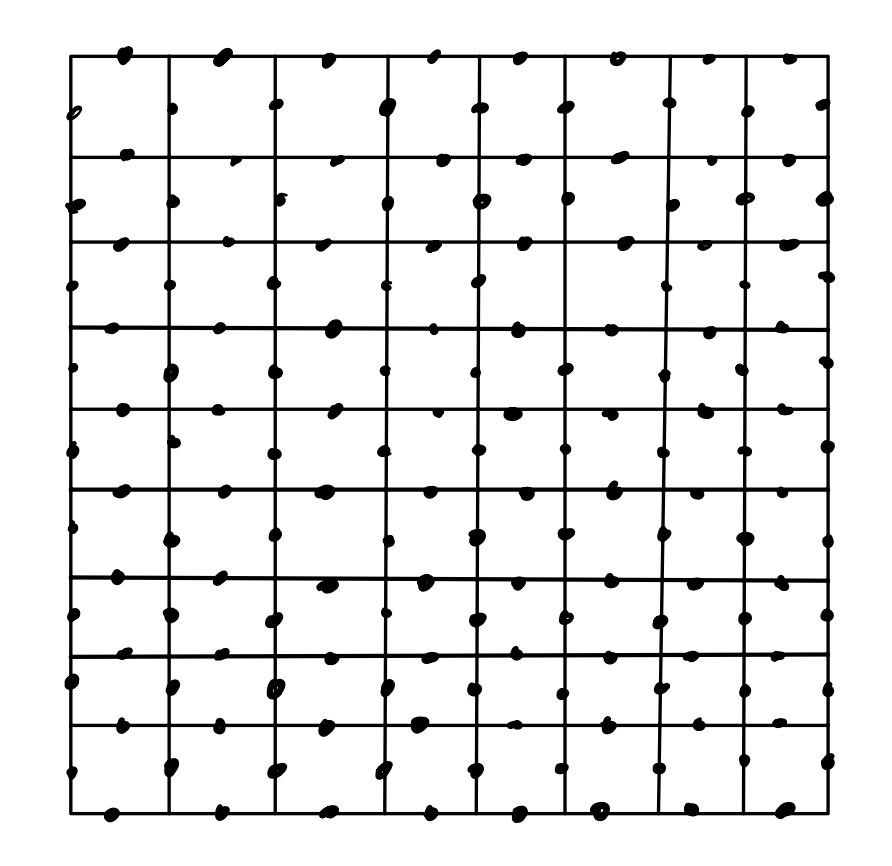
\includegraphics[scale=0.35]{Lectures/Images/lec6-lattice.png}
\end{center}

It is convenient to define two orthonormal basis for each edge, $\set{\uparrow\ket{g}}$ and $\set{\downarrow\ket{g}}$ where $g \in G$. The $\uparrow/\downarrow$ correspond to the orientation of the link. The relationship between these two bases are very simple:
\begin{equation}
    \uparrow\ket{g} = \downarrow\ket{g^{-1}}
\end{equation}
For example:

\begin{center}
    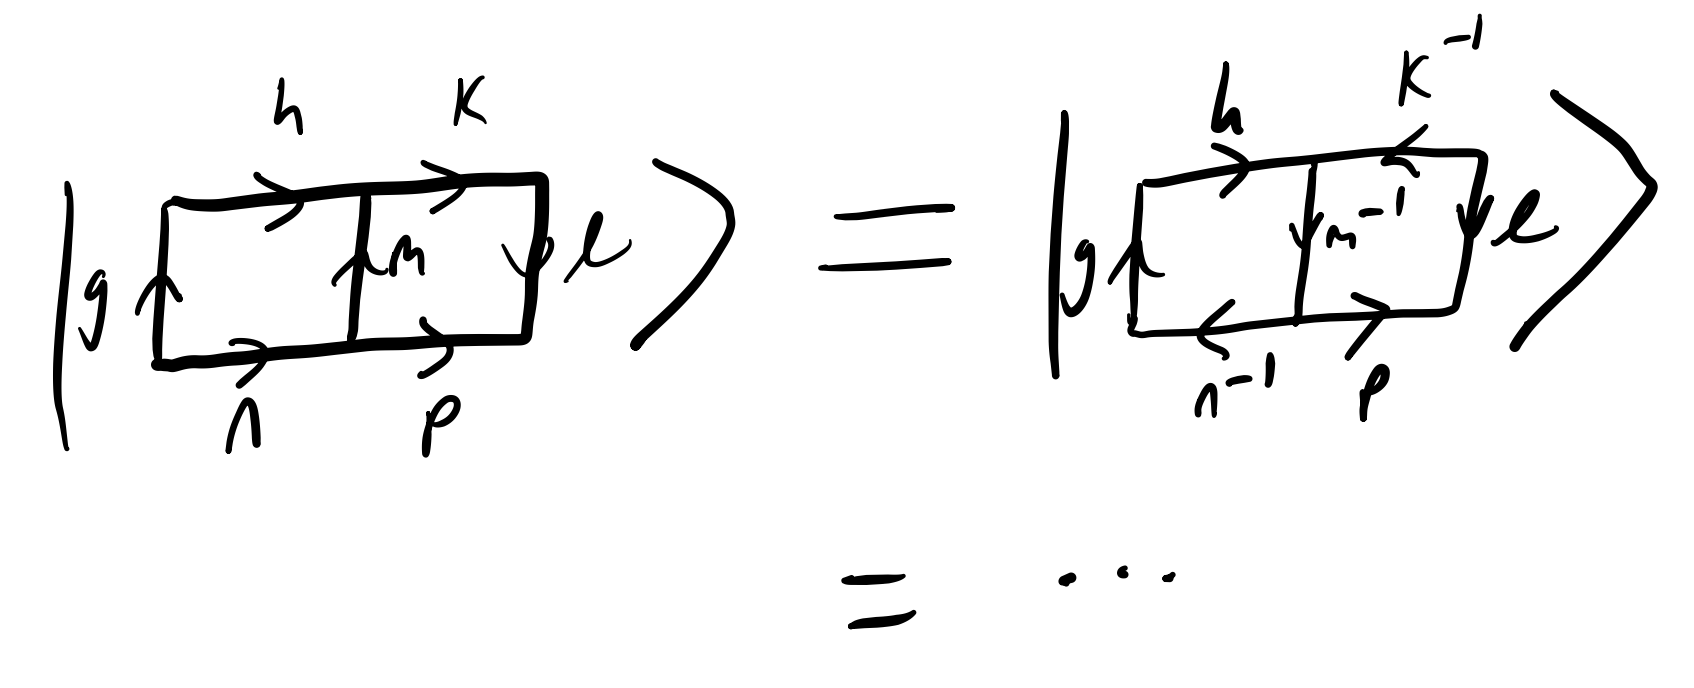
\includegraphics[scale=0.35]{Lectures/Images/lec6-inverse.png}
\end{center}

We're out of time for today, but it's worth noting that quantum double model with group $G$ is related to $G$-gauge theory; just written in a more concrete way. In such a gauge theory, to transport a charge in the gauge theory along a link you use unitary $g/g^{-1}$ depending on which direction you want to transport it.
